\section{Results}
The tolerance for some of the subjects is not representative, as the examiner was not able to apply enough force with the algometer to reach the subjects' tolerance, thus those subjects were excluded. 
Therefore the results are based on 32 subjects, 15 subjects in the treatment and 17 subjects in the control group. 

The threshold and tolerance increases for both, treatment and control group, between the measurements. The Improvement in threshold and tolerance is illustrated in Figure \ref{fig:barplot}. 

\begin{figure}[H]
\centering
%\caption{} \vspace{-.25cm}
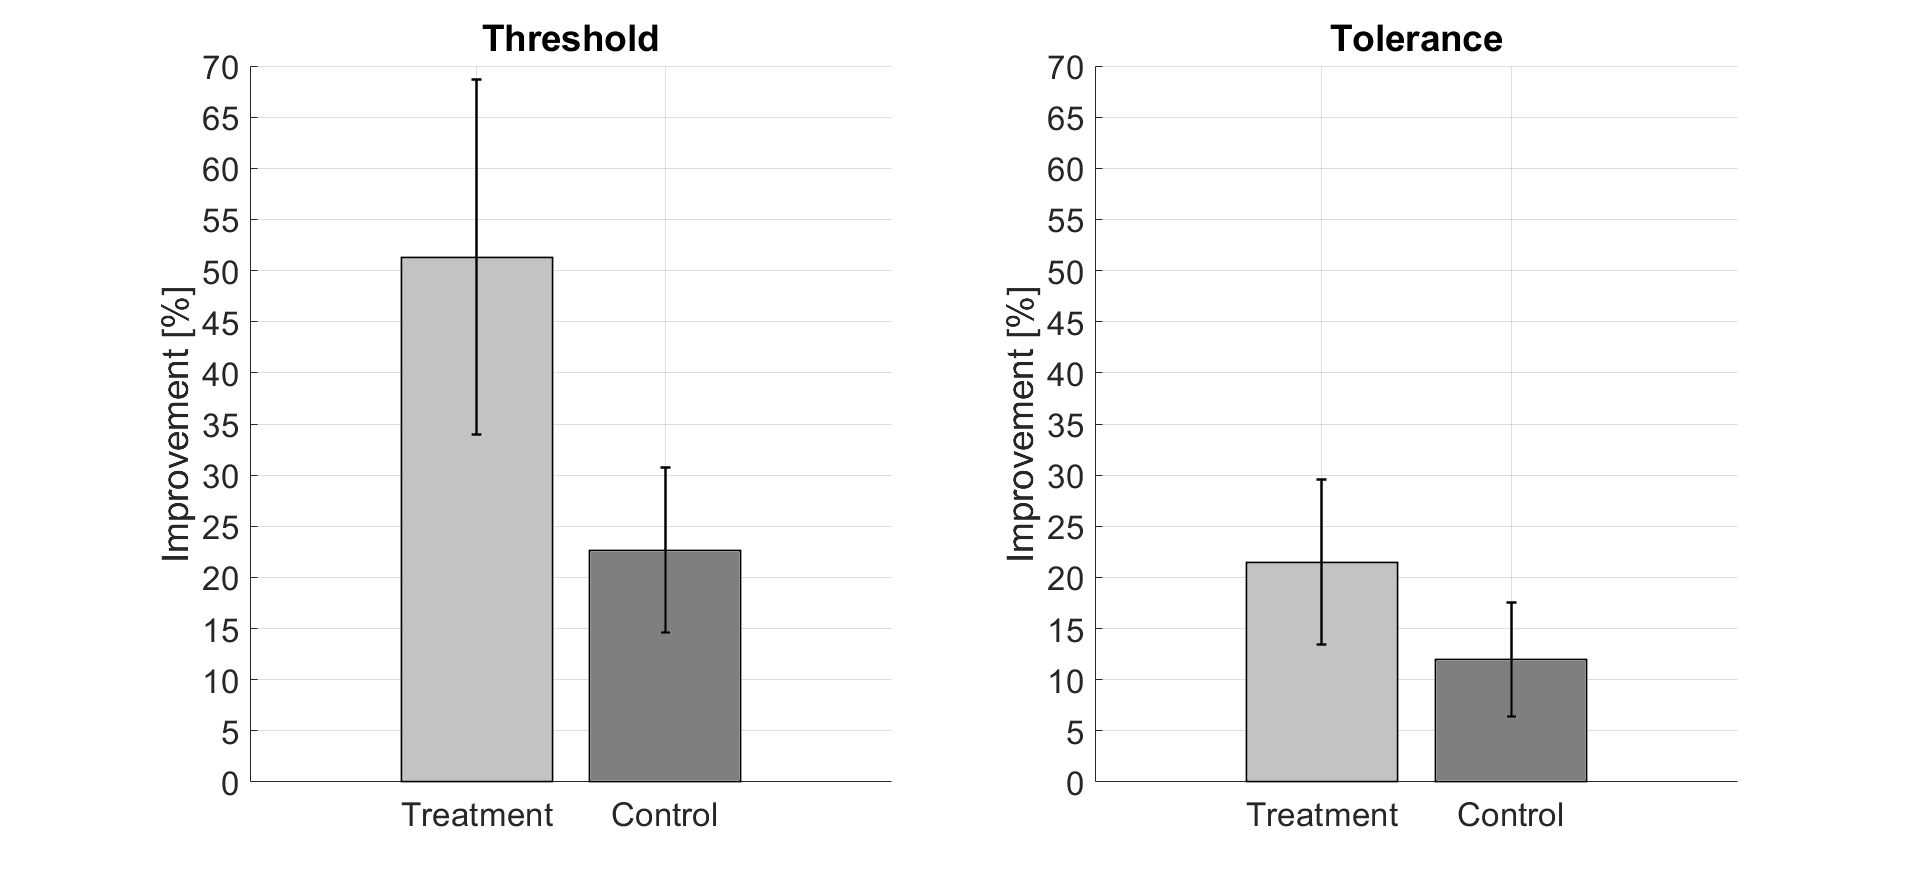
\includegraphics[width=1\columnwidth]{../figures/barplot.png}
\caption{Improvement for threshold (left) and tolerance (right) with associated standard error for treatment group (light grey) and control group (dark grey).}
\label{fig:barplot}
\end{figure} 

The Shapiro-Wilk test showed a normal distribution ($\alpha$ > 0.05) and the Levene's test showed equal variances ($\alpha$ > 0.05) for the threshold and tolerance Pre and Post for both, treatment and control group. Therefore the two-way mixed ANOVA was applied. Hereby the Pre and Post measurements of threshold and tolerance were compared to assess the within-subjects effect. The treatment and control group were compared to assess the between-subjects effect. The results from the two-way mixed ANOVA are illustrated in Table \ref{table:TWOWAYANOVA1} for threshold and Table \ref{table:TWOWAYANOVA2} for the tolerance. 

\begin{table}[ht]
\caption{Two-way mixed ANOVA for the threshold Pre and Post for treatment and control group. P-values marked with an asterisk indicate significant difference. F-value and degree of freedom (df) are illustrated as well.}
\centering
\begin{tabular}{l c c c}
\toprule
\multicolumn{4}{c}{\textbf{Within-Subjects Effect}} \\
\midrule
& \textbf{df} &\textbf{F} & \textbf{Sig} \\ [0.5ex] % inserts table %heading
Measurement & 1 & 13.052 &  0.001* \\
Measurement x Group & 1 & 0.451 & 0.507 \\
\toprule
\multicolumn{4}{c}{\textbf{Between-Subjects Effect}} \\
\midrule 
& \textbf{df} & \textbf{F} & \textbf{Sig} \\ [0.5ex] % inserts table %heading
Group & 30 & 1.492 &  0.231 \\
\hline
\end{tabular}
\label{table:TWOWAYANOVA1}
\end{table}

The test indicates that there is a significant main effect between Pre and Post of the threshold measurements (within-subject effect, Measurement), F(1,30) = 13.051, p = 0.001. However, no significant main effect is seen between the treatment and control group for threshold (between-subjects effect, Group), F(1,30) = 1.492, p = 0.231 nor a significant main interaction between measurements and group (within-subjects effect, Measurement x Group), F(1,30) = 0.451, p = 0.507. 

\begin{table}[ht]
\caption{Two-way mixed ANOVA for the tolerance Pre and Post for treatment and control group. P-values marked with an asterisk indicate significant difference. F-value and degree of
freedom (df) are illustrated as well.}
\centering
\begin{tabular}{l c c c}
\toprule
\multicolumn{4}{c}{\textbf{Within-Subjects Effect}} \\
\midrule  
& \textbf{df} & \textbf{F} & \textbf{Sig} \\ [0.5ex] % inserts table %heading
Measurement & 1 &  8.918 &  0.006* \\
Measurement x Group & 1 & 0.532 & 0.472 \\
\toprule
\multicolumn{4}{c}{\textbf{Between-Subjects Effect}} \\
\midrule
 & \textbf{df} & \textbf{F} & \textbf{Sig} \\ [0.5ex] % inserts table %heading
Group & 30 & 3.289 &  0.080 \\
\hline
\end{tabular}
\label{table:TWOWAYANOVA2}
\end{table}

\noindent
The test indicates that there is a significant main effect between Pre and Post of the tolerance measurements (within-subject effect, Measurement), F(1,30) = 8.981, p=0.006. However, no significant main effect is seen between the treatment and control group for threshold (between-subjects effect, Group), F(1,30) = 3.289, p = 0.080 nor a significant main interaction between  measurements and group (within-subjects effect, Measurement x Group), F(1,30) = 0.532, p = 0.472.

The Shapiro-Wilk test showed a normal distribution ($\alpha$ > 0.05) and an unequal variance (p = 0.013) for the Improvement in threshold and tolerance for both groups. Therefore the t-test was applied. The results from the t-test are illustrated in Table \ref{table:TTEST}. 

\begin{table}[ht]
\caption{T-test for threshold and tolerance Improvement for treatment and control group. P-values marked with an asterisk indicate significant difference.}
\centering
\begin{tabular}{c c}
\toprule
\textbf{Threshold} & \textbf{Tolerance} \\
\midrule
 0.149 &  0.330 \\
\hline
\end{tabular}
\label{table:TTEST}
\end{table}

\noindent
The test indicates that there is no significant difference in Improvement in threshold and tolerance between the groups.